\section{Durchführung}
\label{sec:Durchführung}
Der Aufbau des Versuches ist in folgender Abbildung schematisch dargestellt.
  \begin{figure}[H]
    \centering
      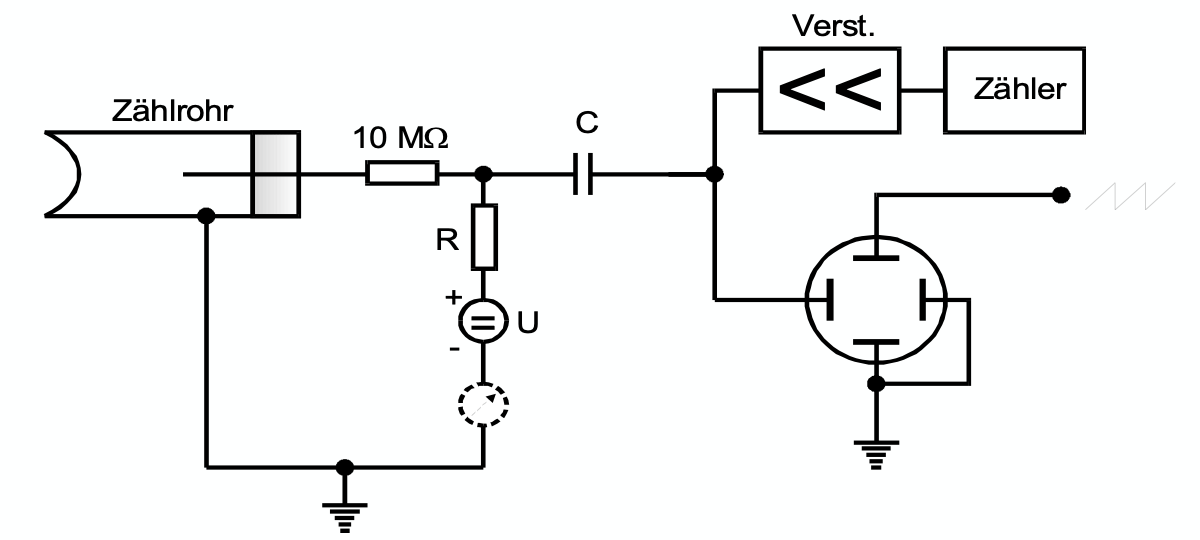
\includegraphics[scale=0.6]{content/AufbauV703.png}
      \caption{Der Versuchsaufbau. Quelle:\cite{AP01}}
      \label{fig:aufbau3}
  \end{figure}
\noindent
\subsection{Aufnahme der Charakteristik des Zählrohres}
    Die Ladung $Q$, die auf dem Zähldraht innerhalb des Zählrohres aufgenommen wird, fließt über den
    Widerstand $R$. Dabei entsteht eine Spannung, die mit dem Kondensator ausgekoppelt und dann
    mithilfe des Verstärkers vergößert wird. Die vergößerte Spannung wird dann mit dem Oszillographen
    sichtbar gemacht. In Schritten von $\increment U = 10 \si{\volt}$ wurde die Anzahl der Zerfälle
    innerhalb eines Zeitintervalls aufgenommen. Um sicherzustellen, dass die Totzeit die Messung nicht
    beeinflusst, wurde mit einer Integrationszeit von $t = 60 \si{\second}$ gearbeitet. Der
    Zählrohrstrom wird alle $\SI{50}{\volt}$ am Amperemeter abgelesen.
\subsection{Messung der Totzeit mit dem Oszillographen}
  Mithilfe der Visualisierung durch das Oszilloskop wurde die Totzeit abgeschätzt, indem die Zeit
  zwischen dem ersten und dem zweiten Puls abgelesen wird. Die Abschätzung erfolgte anhand folgender
  Abbildung.
  \begin{figure}[H]
    \centering
      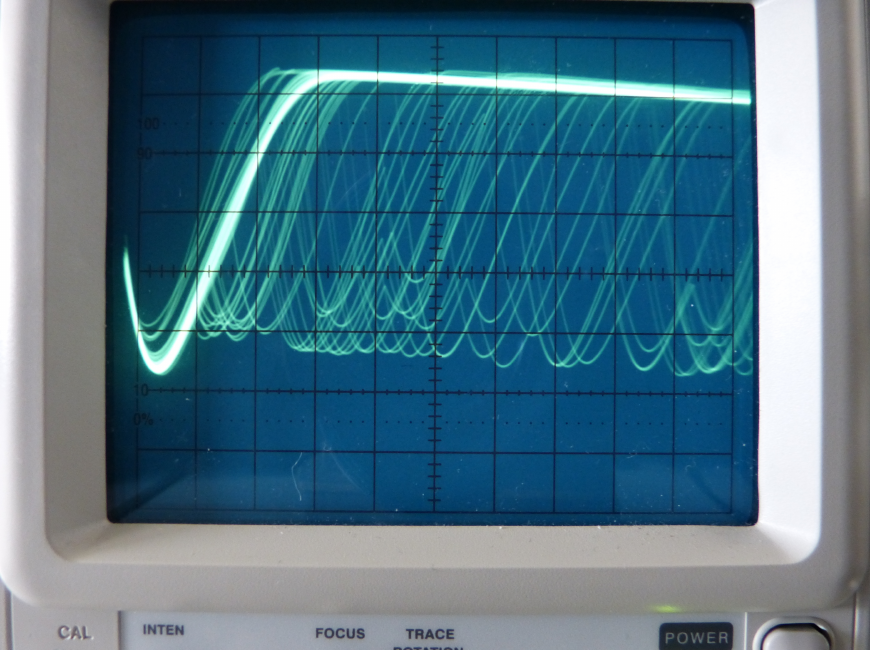
\includegraphics[scale=0.3]{content/Osz.png}
      \caption{Die Visualisierung durch den Oszillographen. Quelle:\cite{AP02}}
      \label{fig:totzeit1}
  \end{figure}
\subsection{Messung der Totzeit mit der Zwei-Quellen-Methode}
  Um die Totzeit mit der Zwei-Quellen-Methode zu bestimmen, wurde die $_{204}Tl$-Quelle näher an das
  Zählrohr heran bewegt, um eine Korrektur der Totzeit vorzunehmen. Für eine genauere Messung wurde
  die Messzeit auf $t = \SI{120}{\second}$ erhöht. Die Zählraten $N_{1}$, $N_{2}$ und $N_{1+2}$ wurden
  gemessen. In der folgenden Abbildung ist der Aufbau zur Bestimmung der Totzeit mit der Zwei-Quellen-
  Methode zu erkennen.
  \begin{figure}[H]
    \centering
      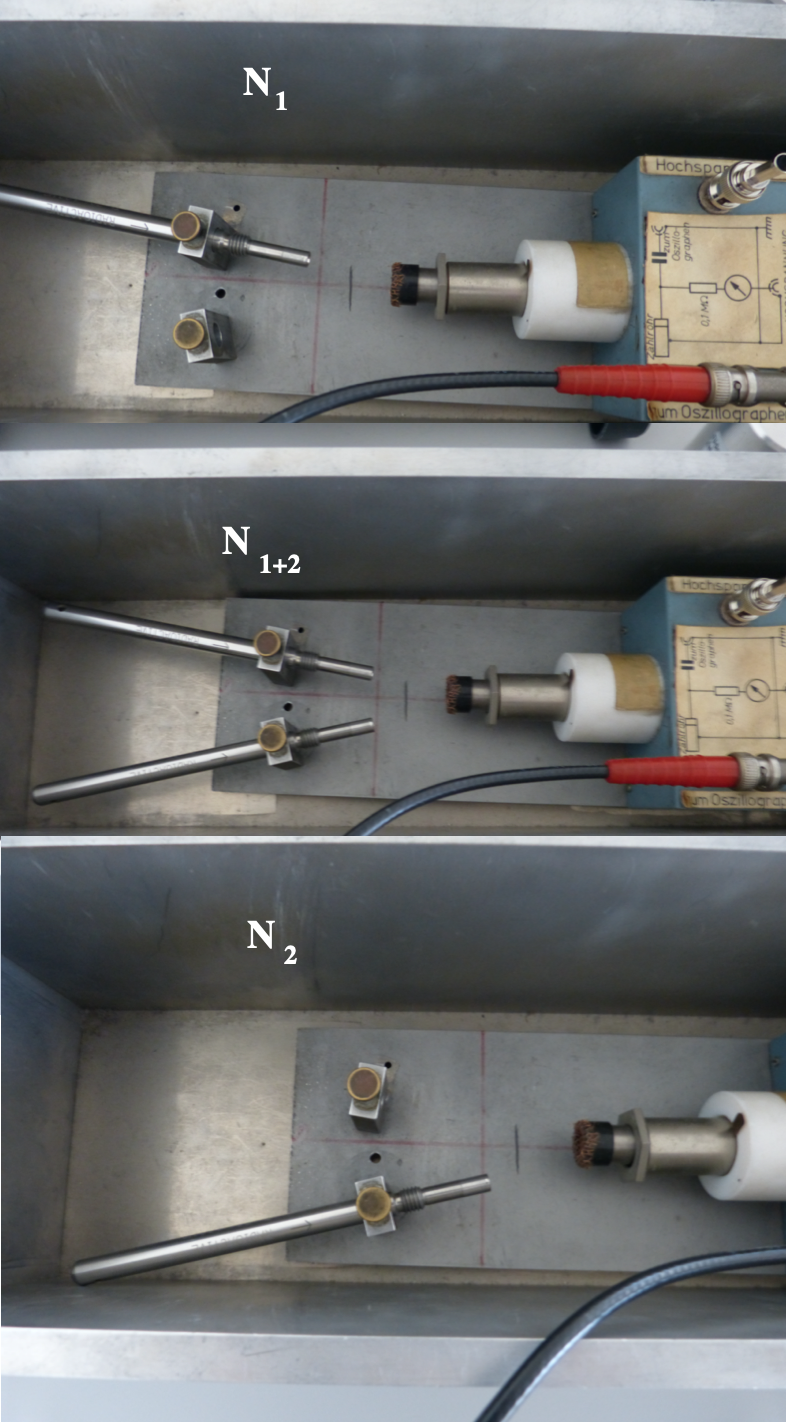
\includegraphics[scale=0.3]{content/totzeit2.png}
      \caption{Der Aufbau zur Messung der Zählraten für die Bestimmung der Totzeit. Quelle:\cite{AP02}}
      \label{fig:totzeit2}
  \end{figure}
